\documentclass{article}

\usepackage[latin1]{inputenc}
\usepackage{verbatim}
\usepackage{tikz}
\usepackage{tikz-3dplot}
\usepackage{pgfplots}
\usepackage{graphicx}
\graphicspath{ {./Pics/} }
\pgfplotsset{compat=1.15}
\usepackage{amsmath}
\usetikzlibrary{datavisualization}
\usetikzlibrary{datavisualization.formats.functions}

\begin{document}
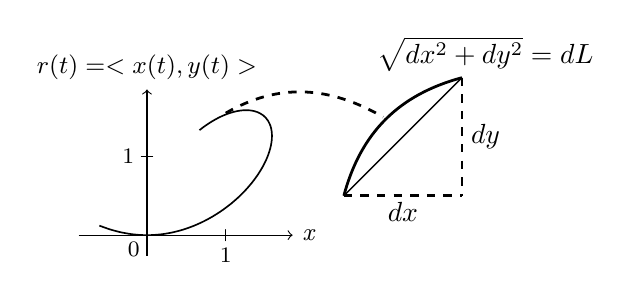
\begin{tikzpicture}
\datavisualization [school book axes,
                    visualize as smooth line,
                    y axis={label={$r(t)=<x(t),y(t)>$}},
                    x axis={label} ]

data [format=function] {
      var t : interval[-.2:2] samples 51;
      func x = 3*(\value t)/(1 + (\value t)^3);
      func y = 3*(\value t)^2/(1 + (\value t)^3);
      };
      \coordinate (P) at (1,1.55);
      \coordinate (Q) at (3,1.5);
      \coordinate (M) at (2.5,0.5);
      \coordinate (O) at (4,2);
      \draw[line width=1pt, dashed] (P) to[out=30, in=150] (Q);
      \draw[line width=1pt] (M) to[out=75, in =195] (O);
       \draw[line width=1pt,black, dashed](M)--(4,0.5);
       \draw[line width=1pt,black, dashed](O)--(4,0.5);
       \draw[line width=0.5pt](M)--(O);
       \node at (4.3,1.25) {$dy$};
       \node at (3.25, 0.3) {$dx$};
       \node at (4.3, 2.3) {$\sqrt{dx^2+dy^2} = dL$};
\end{tikzpicture}

\begin{gather*}
   \frac{dx}{dt} = f'(t)
   \\
   dx = f'(t)dt, dy = g'(t)dt
   \\
   dL = \sqrt{dx^2+dy^2} = \sqrt{(f'(t)dt)^2+(g'(t)dt)^2} = \sqrt{(\frac{dx}{dt})^2 + \frac{dy}{dt})^2}
   \\
   L = \int dL = \int_{a}^{b} \sqrt{(\frac{dx}{dt})^2 + \frac{dy}{dt})^2} = \int_{a}^{b} |r'(t)|dt
   \\
   s(t) = \int_{a}^{b} |r'(t)|dt
\end{gather*}


If $\vec{a}\cdot\vec{b} = \vec{a}\cdot\vec{c}$, that does not mean that $\vec{b} = \vec{c}$ because two separate vectors can have the same horizontal component


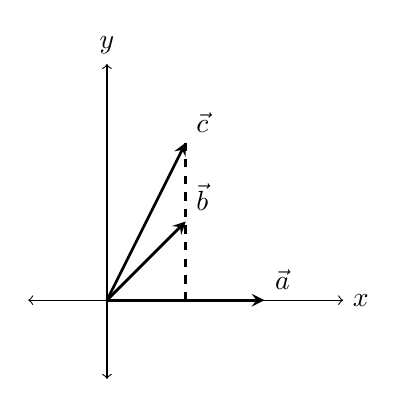
\begin{tikzpicture}
  \draw[<->] (-1,0)--(3,0) node[right]{$x$};
  \draw[<->] (0,-1)--(0,3) node[above]{$y$};
  \draw[line width=1pt,black, -stealth](0,0)--(1,1) node[anchor=south west]{$\vec{b}$};
  \draw[line width=1pt,black,-stealth](0,0)--(1,2) node[anchor=south west]{$\vec{c}$};
  \draw[line width=1pt,black,-stealth](0,0)--(2,0) node[anchor=south west]{$\vec{a}$};
  \draw[line width=1pt,black, dashed](1,0)--(1,2);
\end{tikzpicture}

Also, if $\vec{a}\times\vec{b} = \vec{a}\times\vec{c}$, $\vec{b}$ does not have to be equal to $\vec{c}$ because two separate vectors can have equivalent vertical components

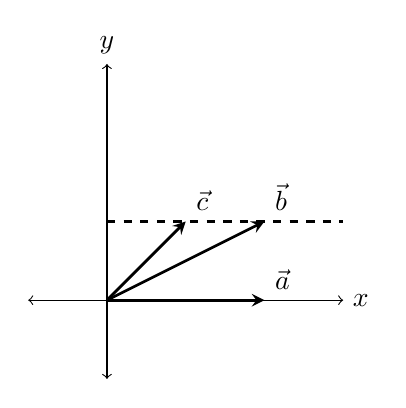
\begin{tikzpicture}
  \draw[<->] (-1,0)--(3,0) node[right]{$x$};
  \draw[<->] (0,-1)--(0,3) node[above]{$y$};
  \draw[line width=1pt,black, -stealth](0,0)--(2,1) node[anchor=south west]{$\vec{b}$};
  \draw[line width=1pt,black,-stealth](0,0)--(1,1) node[anchor=south west]{$\vec{c}$};
  \draw[line width=1pt,black,-stealth](0,0)--(2,0) node[anchor=south west]{$\vec{a}$};
  \draw[line width=1pt,black, dashed](0,1)--(3,1);
\end{tikzpicture}

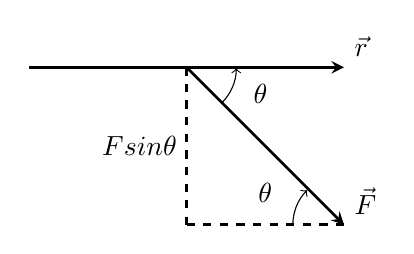
\begin{tikzpicture}
  \draw[line width=1pt,black, -stealth](0,4)--(4,4) node[anchor=south west]{$\vec{r}$};
  \draw[line width=1pt,black,-stealth](2,4)--(4,2) node[anchor=south west]{$\vec{F}$};
  \path (2,4)++(-20:1cm)node{$\theta$};
  \draw[->] (2.45, 3.55) arc (-45:0:0.62cm);
  \draw[line width=1pt,black, dashed](2,4)--(2,2);
  \node[anchor=east] at (2,3) {$Fsin\theta$};
  \draw[line width=1pt,black, dashed](2,2)--(4,2);
  \node at (3, 2.4) {$\theta$};
  \draw[->] (3.35, 2) arc (-180:-225:0.62cm);
\end{tikzpicture}
\begin{gather*}
  \vec{\tau} = (|\vec{r}||\vec{F}|sin\theta)\vec{n}
  \\
  \vec{\tau} = (|\vec{r}||\vec{F}|sin\theta)\vec{n}
  \\
  \vec{a}\times\vec{b} = (|\vec{a}||\vec{b}|sin\theta)\vec{n}
  \\
  \vec{a} = <a_1,a_2,a_3>, \vec{b} = <b_1,b_2,b_3>  
  \\
  \vec{a}\times\vec{b} = 
  \begin{bmatrix} 
     \vec{i} & \vec{j} & \vec{k} \\
     a_1 & a_2 & a_3 \\
     b_1 & b_2 & b_3 
   \end{bmatrix}
   = <(a_2b_3-a_3b_2),-(a_1b_3-a_3b_1),(a_1b_2-a_2b_1)>
\end{gather*}

Directional Derivative


If $g(h) = f(x_o + ha, y_o+hb)$, then by the the definition of a derivative
\begin{gather*}
   g'(0) = \lim_{h\to0}\frac{f(x_o + ha, y_o+hb) - f(x_o,y_o)}{h} = D_u f(x_o,y_o)
\end{gather*}

Or by the chain rule with $x = x_o + ha$ and $y = y_o + hb$
\begin{gather*}
   g'(h) = \frac{\partial f}{\partial x}\frac{dx}{dh} + \frac{\partial f}{\partial y}\frac{dy}{dh}
   \\
   = f_x(x_o,y_o)a + f_y(x_o,y_o)b
   \\
   Duf(x_o,y_o) = \nabla f(x_o,y_o)\cdot\vec{u}
\end{gather*}

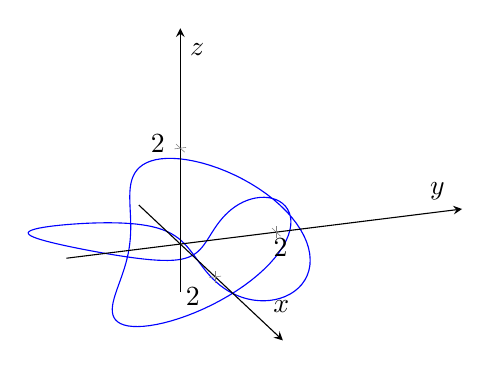
\begin{tikzpicture}
   \begin{axis}[view={70}{20},
                axis lines=center,axis on top,
                xlabel=$x$,ylabel=$y$,zlabel=$z$,
                xtick={2},ytick={2},ztick={2},
                no marks,axis equal,
                xmin=-1,xmax=4,ymin=-1,ymax=4,zmin=-1,zmax=4,
                enlargelimits={upper=0.1}]
     \addplot3+[no markers,samples=800, samples y=0,domain=-400*pi:400*pi,variable=\t]
                                      ({(2+cos(1.5*\t))*cos(\t)},{(2+cos(1.5*\t))*sin(\t)},{sin(1.5*\t});
     %\node at (2,2,2) {$P$}
  \end{axis}
\end{tikzpicture}


Parametric Torus
 
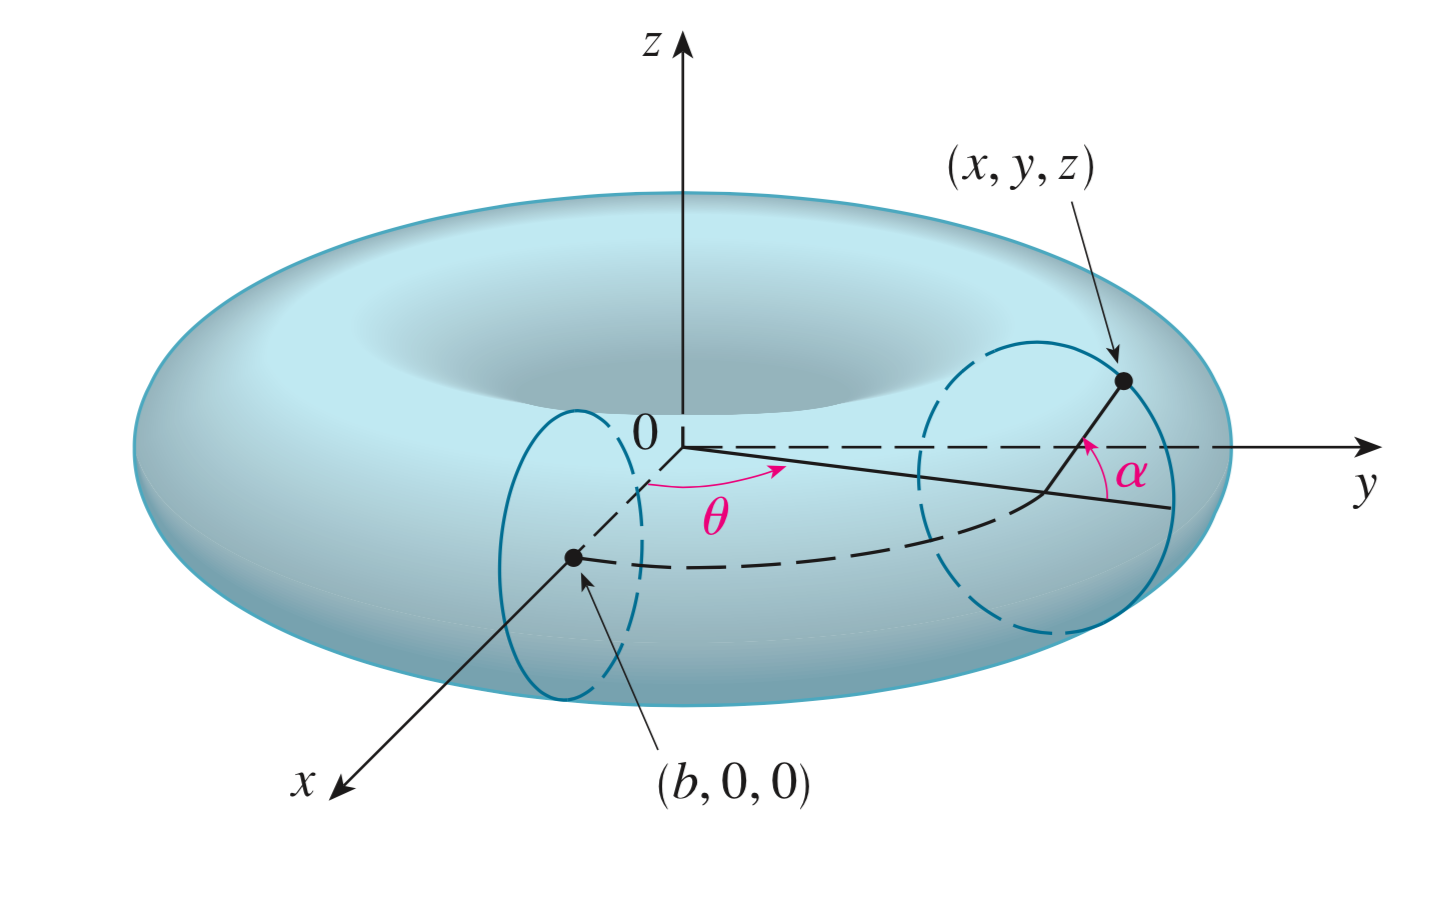
\includegraphics[scale=.15]{torus}
\begin{gather*}
   x = bcos(\theta) + acos(\alpha)cos(\theta)
   \\
   y = bsin(\theta) + acos(\alpha)sin(\theta)
   \\
   z = asin(\alpha)
\end{gather*}

\begin{gather*}
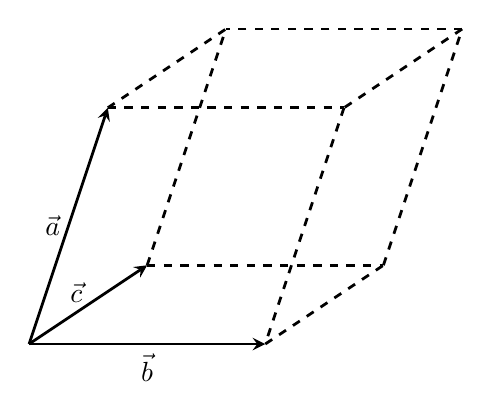
\begin{tikzpicture}
  \draw[line width=1pt,black, -stealth](0,0)--(3,0);
  \draw[line width=1pt,black, -stealth](0,0)--(1.5,1);
  \draw[line width=1pt,black, -stealth](0,0)--(1,3);
  \node at (1.5, -.3){$\vec{b}$};
  \node at (.6, .65){$\vec{c}$};
  \node at (0.3, 1.5){$\vec{a}$};
  \draw[line width=1pt,black, dashed](1,3)--(4,3);
  \draw[line width=1pt,black, dashed](4,3)--(3,0);
  \draw[line width=1pt,black, dashed](3,0)--(4.5,1);
  \draw[line width=1pt,black, dashed](1.5,1)--(4.5,1);
  \draw[line width=1pt,black, dashed](4.5,1)--(5.5,4);
  \draw[line width=1pt,black, dashed](5.5,4)--(4,3);
  \draw[line width=1pt,black, dashed](1,3)--(2.5,4);
  \draw[line width=1pt,black, dashed](1.5,1)--(2.5,4);
  \draw[line width=1pt,black, dashed](5.5,4)--(2.5,4);
\end{tikzpicture}
   V = |\vec{a}cos(\theta)|\vec{b}\times\vec{c}| = \vec{a}\cdot(\vec{b}\times\vec{c})   
\end{gather*}


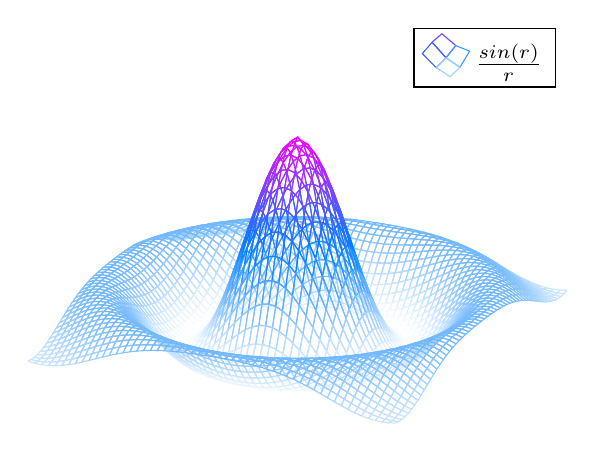
\begin{tikzpicture}
\begin{axis}[
    hide axis,
    colormap/cool,
]
\addplot3[
    mesh,
    samples=55,
    domain=-8:8,
]
{sin(deg(sqrt(x^2+y^2)))/sqrt(x^2+y^2)};
\addlegendentry{$\frac{sin(r)}{r}$}
\end{axis}
\end{tikzpicture}

\begin{gather*}
    \text{Dot Products}
    \\
    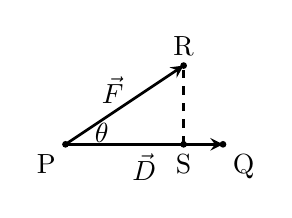
\begin{tikzpicture}
        \draw[line width=1pt, black, -stealth](0,0)--(1.5,1);
        \node[anchor=south] at (0.6, 0.4) {$\vec{F}$};
        \draw[line width=1pt, black, -stealth](0,0)--(2,0);
        \node[anchor=north] at (1,0) {$\vec{D}$};
        \node[anchor= west] at (0.25,0.15) {$\theta$};
        \draw[line width=1pt, black, dashed](1.5,0)--(1.5,1);
        \filldraw[black] (0,0) circle(1pt) node[anchor=north east]{P};
        \filldraw[black] (1.5,0) circle(1pt) node[anchor=north]{S};
        \filldraw[black] (2,0) circle(1pt) node[anchor=north west]{Q};
        \filldraw[black] (1.5,1) circle(1pt) node[anchor=south]{R};
    \end{tikzpicture}
    \\
    |\vec{PS}|=|\vec{F}|cos\theta
    \\
    W=|\vec{D}||\vec{PS}|=|\vec{D}||\vec{F}|cos\theta=\vec{D}\cdot\vec{F}
    \\
    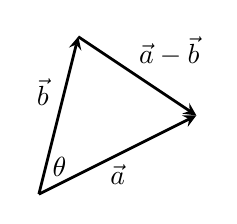
\begin{tikzpicture}
        \draw[line width=1pt, black, -stealth](0,0)--(0.5,2);
        \node[anchor=south east] at (0.25, 1) {$\vec{b}$};
        \draw[line width=1pt, black, -stealth](0,0)--(2,1);
        \node[anchor=north] at (1, 0.5) {$\vec{a}$};
        \draw[line width=1pt, black, -stealth](0.5,2)--(2,1);
        \node[anchor=south west] at (1.15, 1.5) {$\vec{a}-\vec{b}$};
        \node[anchor=south west] at (0.05, 0.1) {$\theta$};
    \end{tikzpicture}
    \\
    |\vec{a}-\vec{b}|^2=|\vec{a}|^2+|\vec{b}|^2-2|\vec{a}||\vec{b}|cos\theta
    \\
    \vec{a}\cdot\vec{b}=\frac{|\vec{a}|^2+|\vec{b}|^2-|\vec{a}-\vec{b}|^2}{2}
    \\
    \vec{a}\cdot\vec{b}=a_1b_1+a_2b_2+a_3b_3
\end{gather*}

%Angle Definitions
%-----------------

%set the plot display orientation
%synatax: \tdplotsetdisplay{\theta_d}{\phi_d}
\tdplotsetmaincoords{60}{110}

%define polar coordinates for some vector
%TODO: look into using 3d spherical coordinate system
\pgfmathsetmacro{\rhovec}{.8}
\pgfmathsetmacro{\thetavec}{30}
\pgfmathsetmacro{\phivec}{60}

\begin{gather*}
\text{Spherical Coordinate System}
\\
%start tikz picture, and use the tdplot_main_coords style to implement the display 
%coordinate transformation provided by 3dplot
\begin{tikzpicture}[scale=5,tdplot_main_coords]
%set up some coordinates 
%-----------------------
\coordinate (O) at (0,0,0);
%determine a coordinate (P) using (\rho,\theta,\phi) coordinates.  This command
%also determines (Pxy), (Pxz), and (Pyz): the xy-, xz-, and yz-projections
%of the point (P).
%syntax: \tdplotsetcoord{Coordinate name without parentheses}{r}{\theta}{\phi}
\tdplotsetcoord{P}{\rhovec}{\thetavec}{\phivec}
%draw figure contents
%--------------------
%draw the main coordinate system axes
\draw[thick,->] (0,0,0) -- (1,0,0) node[anchor=north east]{$x$};
\draw[thick,->] (0,0,0) -- (0,1,0) node[anchor=north west]{$y$};
\draw[thick,->] (0,0,0) -- (0,0,1) node[anchor=south]{$z$};
%draw a vector from origin to point (P) 
\draw[-stealth,color=blue] (O) -- (P);
\node[anchor=south] at (1,0.6,1.3) {$P(x,y,z)$};
\node[anchor=south] at (1,0.6,1.2) {$P(\rho,\theta,\phi)$};
%draw projection on xy plane, and a connecting line
\draw[dashed, color=blue] (O) -- (Pxy);
\node[anchor=north] at (0.12,0.37,0) {$r=\rho sin\theta$};
\draw[dashed, color=blue] (P) -- (Pxy);
\node[anchor=west] at (0.5, 0.45, 0.5) {$z=\rho cos\theta$};
\node[anchor=west] at (0.2, 0.17, 0.5) {$\rho$};
%draw the angle \phi, and label it
%syntax: \tdplotdrawarc[coordinate frame, draw options]{center point}{r}{angle}{label options}{label}
\tdplotdrawarc{(O)}{0.2}{0}{\phivec}{anchor=north}{$\theta$}
%set the rotated coordinate system so the x'-y' plane lies within the
%"theta plane" of the main coordinate system
%syntax: \tdplotsetthetaplanecoords{\phi}
\tdplotsetthetaplanecoords{\phivec}
%draw theta arc and label, using rotated coordinate system
\tdplotdrawarc[tdplot_rotated_coords]{(0,0,0)}{0.3}{0}{\thetavec}{anchor=south}{$\phi$}
%WARNING:  coordinates defined by the \coordinate command (eg. (O), (P), etc.)
%cannot be used in rotated coordinate frames.  Use only literal coordinates.  
\end{tikzpicture}
    \\
    r=\rho sin\theta
    \\
    x=rcos\theta=\rho cos\theta sin\phi
    \\
    y=rsin\theta=\rho sin\theta sin\phi
    \\
    z=\rho cos\theta
    \\
    \rho^2=x^2+y^2+z^2
\end{gather*}

\begin{gather*}
    \text{Distance to a Line}
    \\
    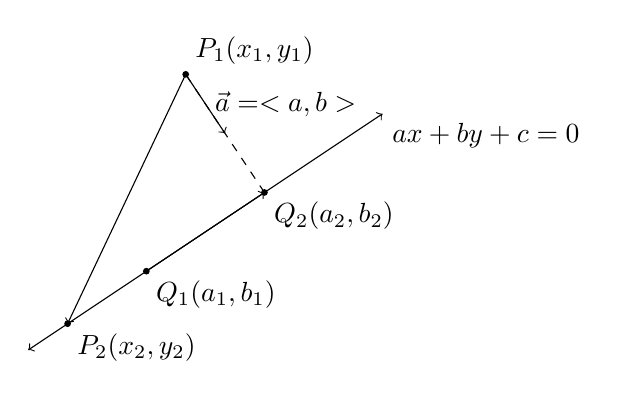
\begin{tikzpicture}
        \draw[<->](-1.5,-1)--(3,2);
        \filldraw[black] (-1,-2/3) circle(1pt) node[anchor=north west] {$P_2(x_2,y_2)$};
        \node[anchor=north west] at (3,2) {$ax+by+c=0$};
        \draw[->](0,0)--(1.5,1);
        \filldraw[black] (0,0) circle(1pt) node[anchor=north west] {$Q_1(a_1,b_1)$};
        \filldraw[black] (1.5,1) circle(1pt) node[anchor=north west] {$Q_2(a_2,b_2)$};
        \draw[dashed](1.5,1)--(0.5,2.5);
        \filldraw[black] (0.5,2.5) circle(1pt) node[anchor=south west] {$P_1(x_1,y_1)$};
        \draw[->](0.5,2.5)--(-1,-2/3);
        \draw[->](0.5,2.5)--(1,1.75);
        \node[anchor=west] at (0.75,2.125) {$\vec{a}=<a,b>$};
    \end{tikzpicture}
    \\
    \text{Since the slope of $ax+by+c=0$ is $-\frac{a}{b}$, the slope of a $\bot$ line is $\frac{b}{a}$, therefore $<a,b>\bot$ $\vec{Q_1Q_2}$,}
    \\
    \text{so $<a,b>\cdot<a_2-a_1,b_2-b_1>=0$}
    \\
    \text{Proof:}
    \\
    aa_2-aa_1+bb_2-bb_1=0
    \\
    aa_1+bb_1=-c=aa_2+bb_2
    \\
    aa_2-aa_1+bb_2-bb_1=0
    \\
    \text{The magnitude of the scalar projection of $\vec{P_1P_2}$ onto $\vec{a}$ is the distance between $P_1$ and the line.}
    \\
    |comp_{<a,b>} \vec{P_1P_2}|=\frac{|<x_1-x_2,y_1-y_2>\cdot <a,b>|}{\sqrt{a^2+b^2}}=\frac{|ax_1-ax_2+by_1-by_2|}{\sqrt{a^2+b^2}}
    \\
    =\frac{|ax_1+by_1+c|}{\sqrt{a^2+b^2}}
    \\
    \text{since $-ax_2-by_2=+c$}
\end{gather*}

\begin{gather*}
    \text{Three Space Distances}
    \\
    \sqrt{x^2+y^2+z^2}=D
\end{gather*}

\begin{gather*}
    \text{Derivative of a Space Curve}
    \\
    \frac{dr}{dt}=\vec{r'}=\lim_{h->0}\frac{\vec{r}(t+h)-\vec{r}(t)}{h}
\end{gather*}

\begin{gather*}
    \text{Parallelogram Vector Addition}
    \\
    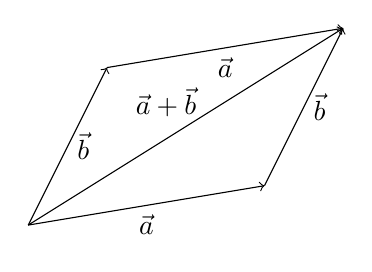
\begin{tikzpicture}
        \draw[->](0,0)--(1,2);
        \draw[->](0,0)--(3,0.5);
        \node[anchor=north] at (1.5,0.25) {$\Vec{a}$};
        \node[anchor=west] at (0.5,1) {$\Vec{b}$};
        \draw[->](1,2)--(4,2.5);
        \draw[->](3,0.5)--(4,2.5);
        \node[anchor=north] at (2.5,2.25) {$\Vec{a}$};
        \node[anchor=west] at (3.5,1.5) {$\Vec{b}$};
        \draw[->](0,0)--(4,2.5);
        \node[anchor=south] at (1.75,1.25) {$\Vec{a}+\Vec{b}$};
    \end{tikzpicture}
\end{gather*}

\begin{gather*}
    \text{Equation of a Line}
    \\
    \begin{tikzpicture}
        \draw[->, line width=1.25pt](0,0)--(1.5,1);
        \node[anchor=south] at (0.8,1) {$\Vec{v}=<a,b>$};
        \filldraw[black] (0,0) circle(1pt) node[anchor=east] {$P_0(x_0,y_0)$};
        \draw[->](0,0)--(6,4);
        \node[anchor=south] at (4,2) {$t\cdot\Vec{v}$};
    \end{tikzpicture}
    \\
    \Vec{r}=P_0+t\Vec{v}=<x_0,y_0>+t<a,b>=<x_0+ta,y_0+tb>
    \\
    x=x_0+ta
    \\
    y=y_0+tb
\end{gather*}

\textbf{Gradient Vectors and Directional Derivative Equations}
\\
\begin {gather*}
    \nabla f(x,y) = <f_x(x,y), f_y(x,y)>
    \\
    D_uf(x,y)= \nabla f(x,y) \cdot u          
\end{gather*}              

\begin{gather*}
\text{Partial Derivatives}
\\
g(x)=f(x,b)
\\
f_x(a,b)=g'(a)
\\
\text{Partial Derivatives using limit definition of a derivative}
\\
f_x(x,y)=lim_{h\xrightarrow{}0} \frac{f(x+h,y)-f(x,y)}{h}
\\
f_y(x,y)=lim_{h\xrightarrow{}0} \frac{f(x,y+h)-f(x,y)}{h}
\end{gather*}

\begin{gather*}
\text{\textbf{Unit Vectors}}
\\
   \text{A unit vector is a vector that has a length of 1.}
   \\
   \text{The unit vector of } \Vec{a} \text{:}
   \\
   \Vec{u}= \frac{\Vec{a}}{|\Vec{a}|}
\end{gather*}

Given $s$ is a level surface with equation $F(x,y,z) = k$, a level surface, of the function $F$, and $P(x_o,y_o,z_o)$ is a point on $s$. $C$ is any curve that lies on $s$ and passes through $P$, and $C$ is described by $r(t) = <x(t), y(t), z(t)>$ with $r_o = <x_o, y_o, z_o>$ corresponding to $P$. Any point on $C$ must satisfy the equation of $F(x(t), y(t), z(t)) = k$.
\begin{gather*}
   \text{Differentiating both sides with the chain rule you get}
   \\
   \frac{\partial{F}}{\partial{x}}\frac{dx}{dt} + \frac{\partial{F}}{\partial{y}}\frac{dy}{dt} + \frac{\partial{F}}{\partial{y}}\frac{dy}{dt} = 0
   \\
   <\frac{\partial{F}}{\partial{x}}, \frac{\partial{F}}{\partial{y}}, \frac{\partial{F}}{\partial{z}}>\cdot<\frac{dx}{dt}, \frac{dy}{dt}, \frac{dz}{dt}> = 0
   \\
   \nabla F\cdot\vec{r'(t)} = 0
   \\
   t = t_o
   \\
   \nabla F(x_o, y_o, z_o)\cdot\vec{r'(t_o)} = 0
   \\
   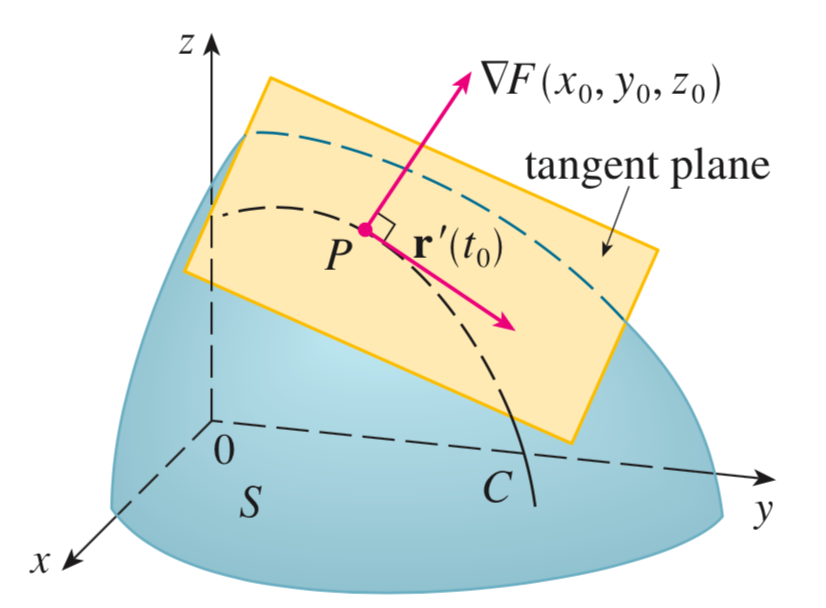
\includegraphics[scale=.2]{tandiag}
\end{gather*}
   So the gradient vector at $P$ is perpindicular to the tangent vector $\vec{r'(t)}$. Given that $F(x(t), y(t), z(t)) = k$ defines a level curve of the surface $S$, then the gradient vector is always perpindicular to all level surfaces. So the normal vector to a level curve is $\nabla F(x_o, y_o, z_o)$. Therefore, the equation of a tangent plane at point $P$ is given by
\begin{gather*}
   F_x(x_o, y_o, z_o)(x-x_o) + F_y(x_o, y_o, z_o)(y-y_o) + F_z(x_o, y_o, z_o)(z-z_o) = 0 
   \\
   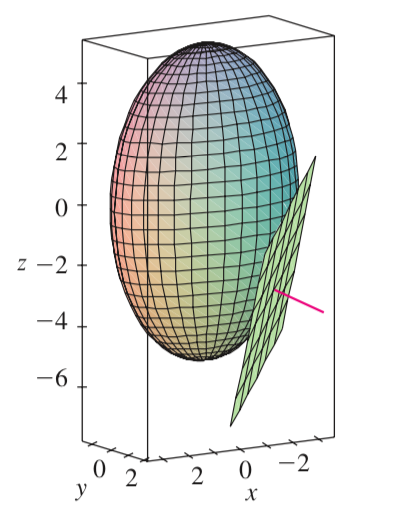
\includegraphics[scale=.25]{tanexample}
\end{gather*}

\begin{gather*}
   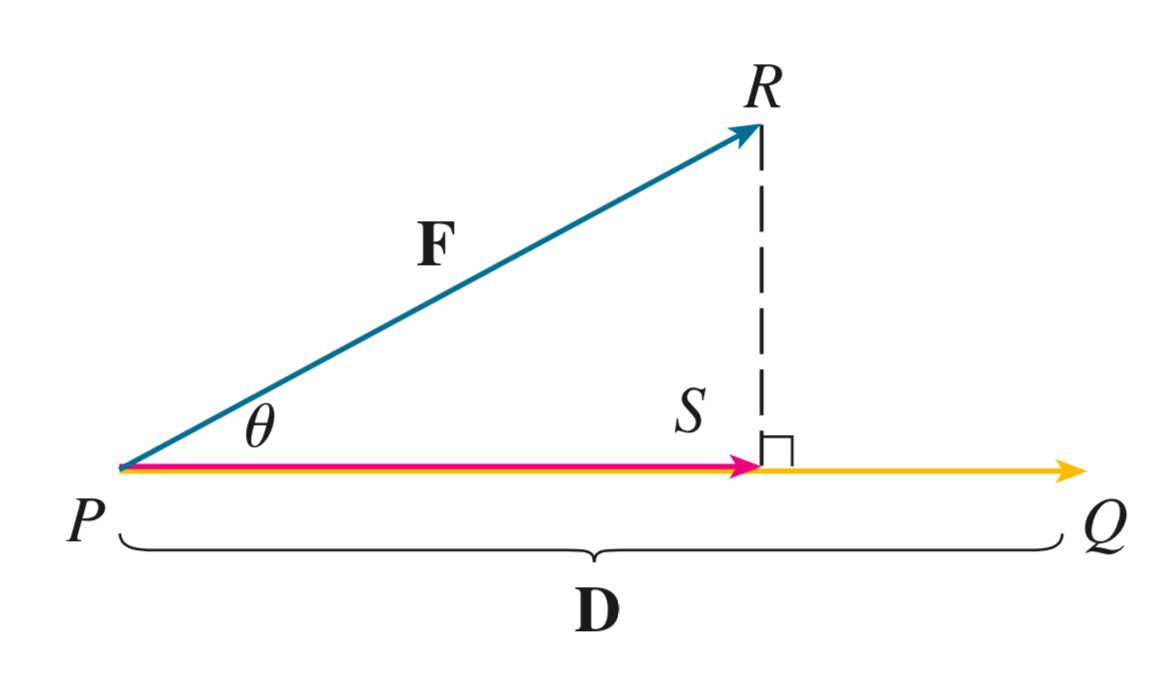
\includegraphics[scale=.2]{work}
   \\
   \boldsymbol{F} = \vec{PR}
   \\
   \boldsymbol{D} = \vec{PQ}
   \\
   \text{The work done by $\bf{F}$ is defined as the magnitude of the displacement, $|\bf{D}|$,}
   \\
   \text{multiplied by the magnitude of the applied force in the direction of the motion}
   \\
   |\vec{PS}| = |\textbf{F} |cos\theta
   \\
   \text{So the work is defined to be }
   W = |\textbf{D}|(|\textbf{F} |cos\theta) = |\textbf{D}||\textbf{F}| cos\theta
\end{gather*}

\begin{gather*}
   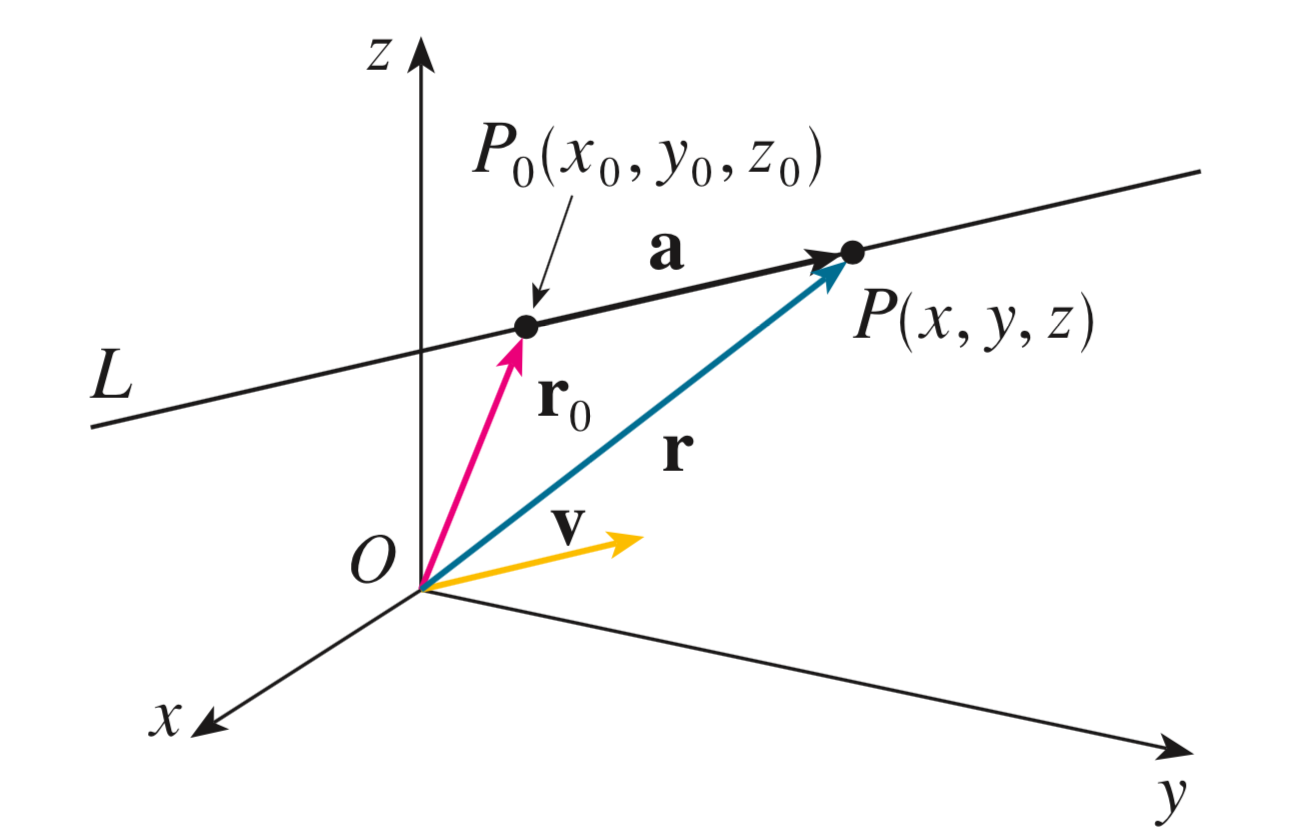
\includegraphics[scale=.2]{linediagram}
   \\
   \vec{r} = \vec{r_o} + t\vec{v}
\end{gather*}

Let $P$ be a point not on the plane that passes through the points $Q,R$ and $S$. Show that the distance $d$ from $P$ to the plane is

\begin{equation*}
   d = \frac{|\bf{a}\cdot(\bf{b}\times\bf{c})|}{|\bf{a}\times\bf{b}|}
\end{equation*}

where $\boldsymbol{a} = \vec{QR}, \boldsymbol{b} = \vec{QS},$ and $\boldsymbol{c} = \vec{QP}$.

The distance is defined as $|\vec{PS}| = d$. But refering to triangle $PQS$, $d = |\vec{PS}| = |\vec{PS}|sin\theta = |\boldsymbol{b}|sin\theta$. But $\theta$ is the angle between $\vec{QP} = \boldsymbol{b}$ and $\vec{QR} = \boldsymbol{a}$. Thus by definition of cross product, $sin\theta = \frac{|\bf{a}\times\bf{b}|}{|\bf{a}||\bf{b}|}$, and so $d = |\boldsymbol{b}|sin\theta = \frac{|\bf{b}||\bf{a}\times\bf{b}|}{|\bf{a}||\bf{b}|}$

\begin{gather*}
   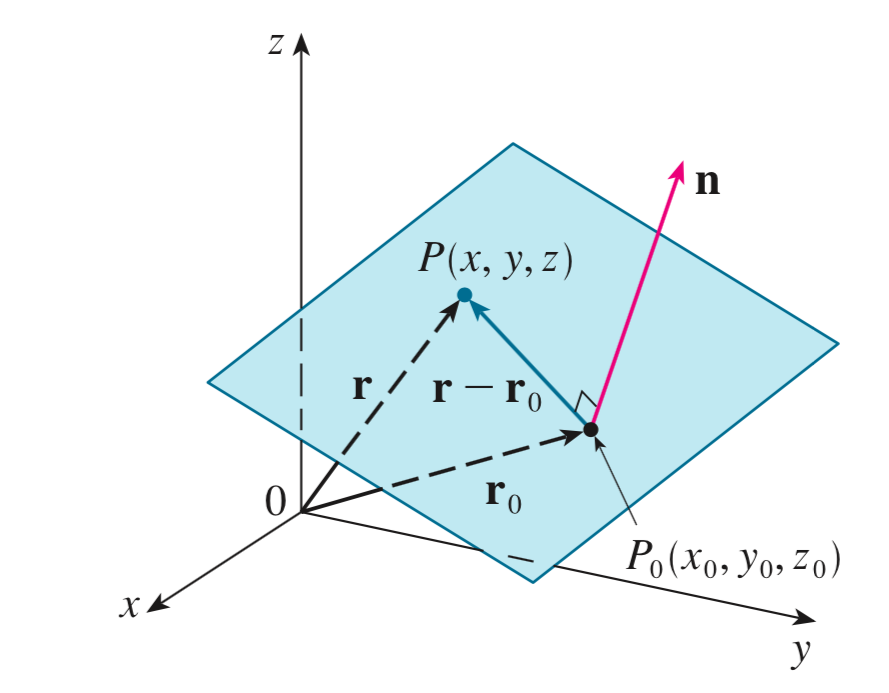
\includegraphics[scale=.2]{planediagram}
   \\
   \boldsymbol{n}\cdot(\boldsymbol{r} - \boldsymbol{r_o}) = 0
   \\
   \boldsymbol{r} = <x,y,z>
   \\
   \boldsymbol{r_o} = <x_o,y_o,z_o>
   \\
   \boldsymbol{n} = <a,b,c>
   \\
   \text{So the equation of a plane is}
   \\
   a(x - x_o) + b(y - y_o) + c(z - z_o) = 0
\end{gather*}

\begin{gather*}
   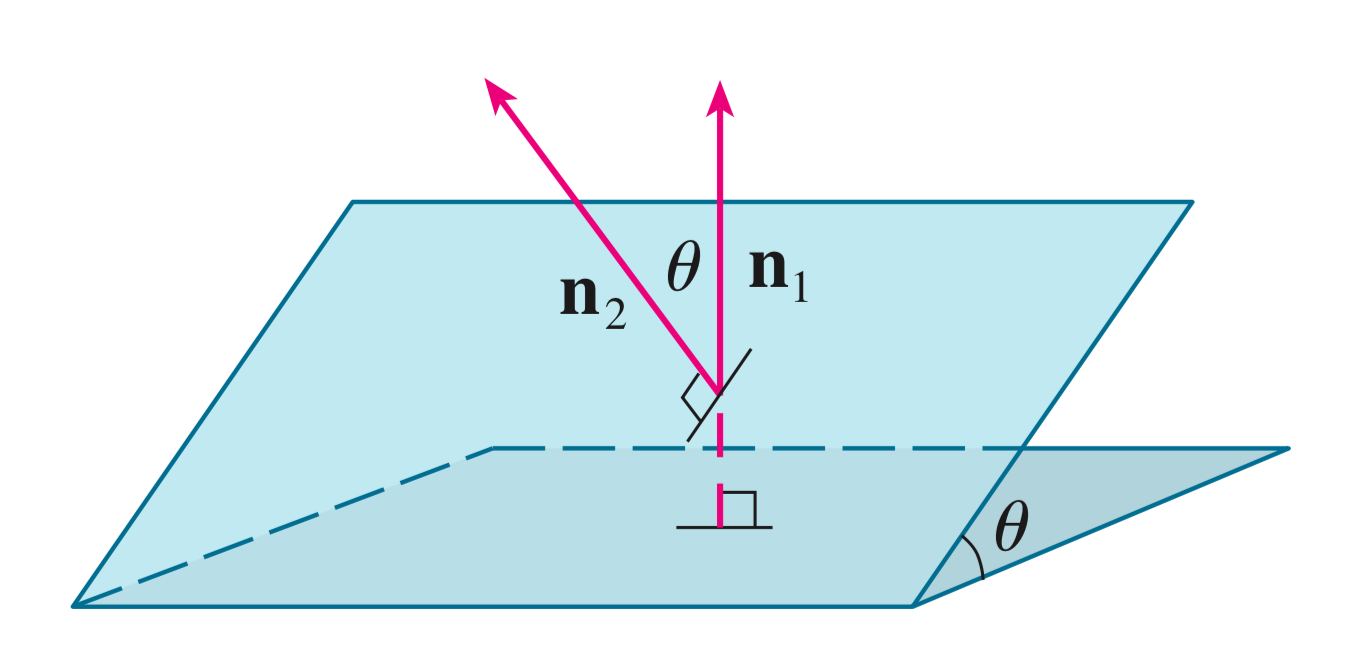
\includegraphics[scale=.2]{planeangle}
   \\
   cos\theta = \frac{\boldsymbol{n}_1\cdot\boldsymbol{n}_2}{|\boldsymbol{n}_1||\boldsymbol{n}_2|}
\end{gather*}

\begin{gather*}
   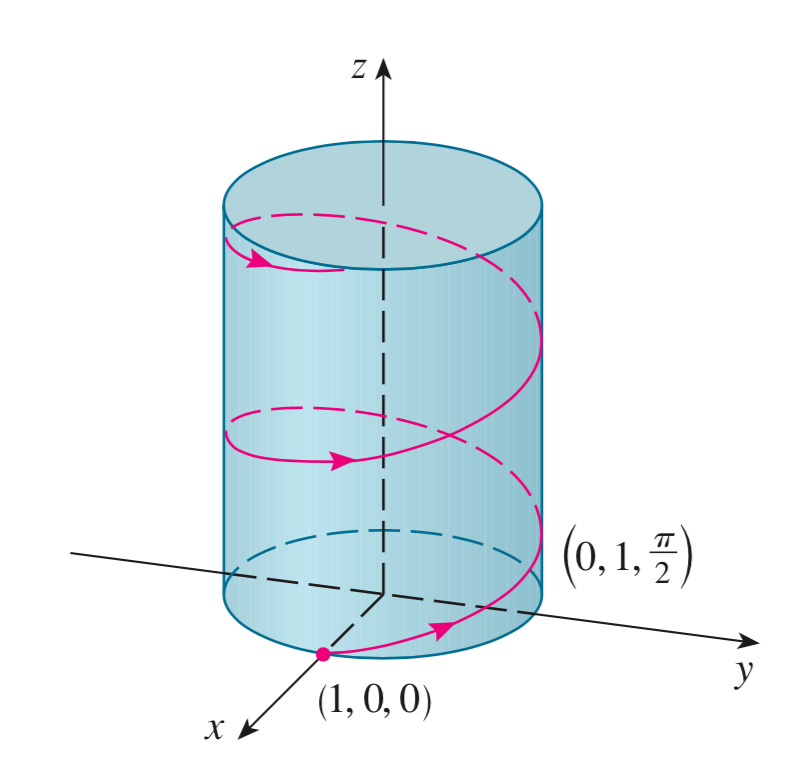
\includegraphics[scale=.2]{helix}
   \\
   \vec{r(t)} = \text{cos } t\boldsymbol{i} + \text{sin }t\boldsymbol{j} + t\boldsymbol{k}
\end{gather*}

\begin{gather*}
   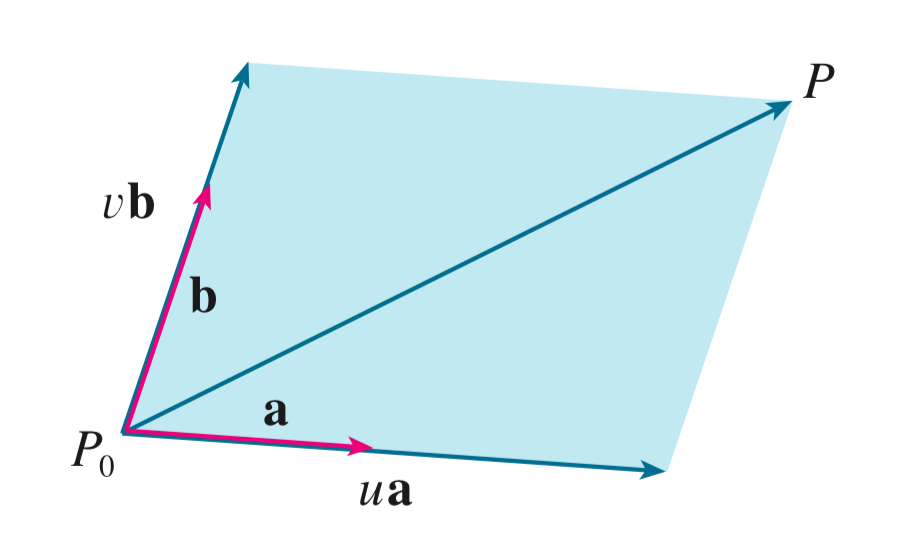
\includegraphics[scale=.15]{nonperp}
   \\
   \boldsymbol{r} = \boldsymbol{r}_o + u\boldsymbol{a} + v\boldsymbol{b}
\end{gather*}

\begin{gather*}
   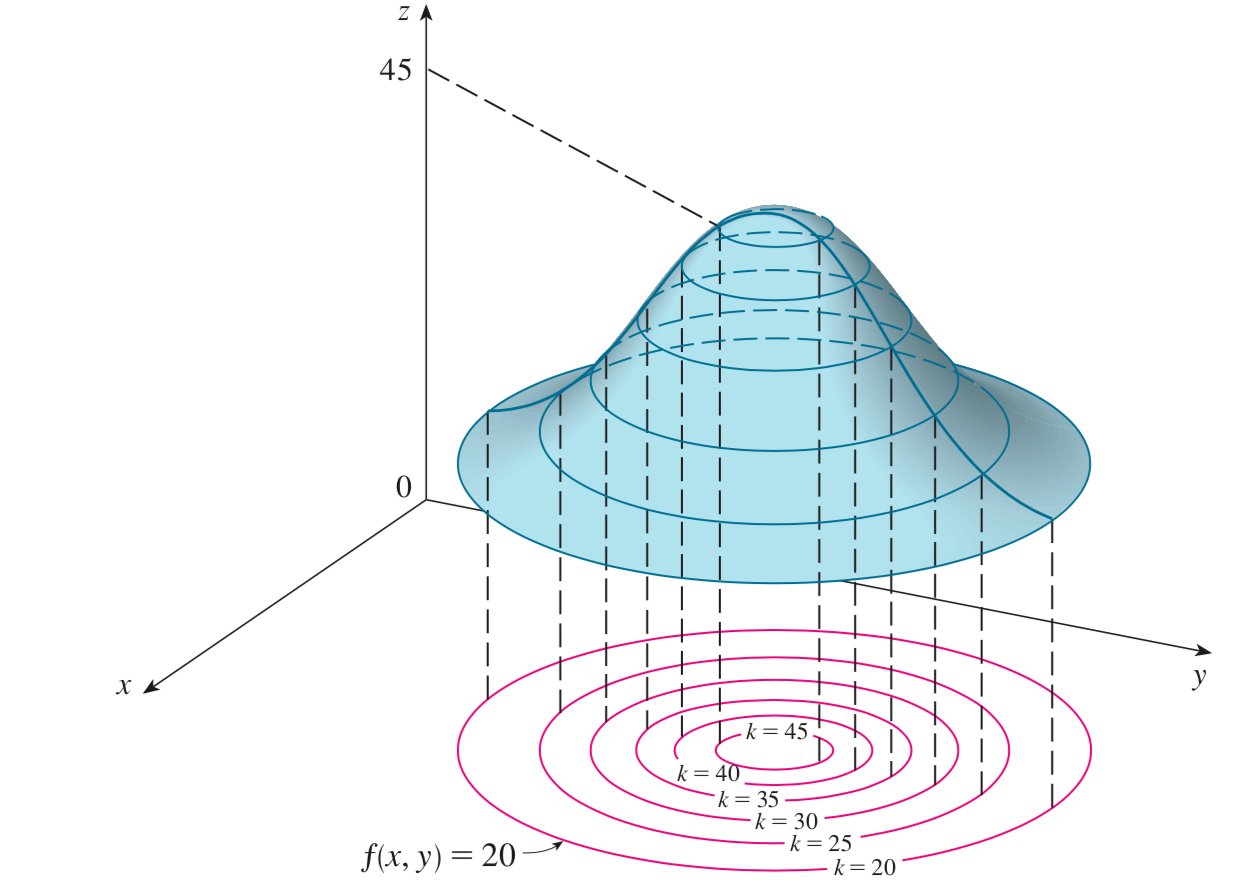
\includegraphics[scale=.2]{contourlines}
   \\
   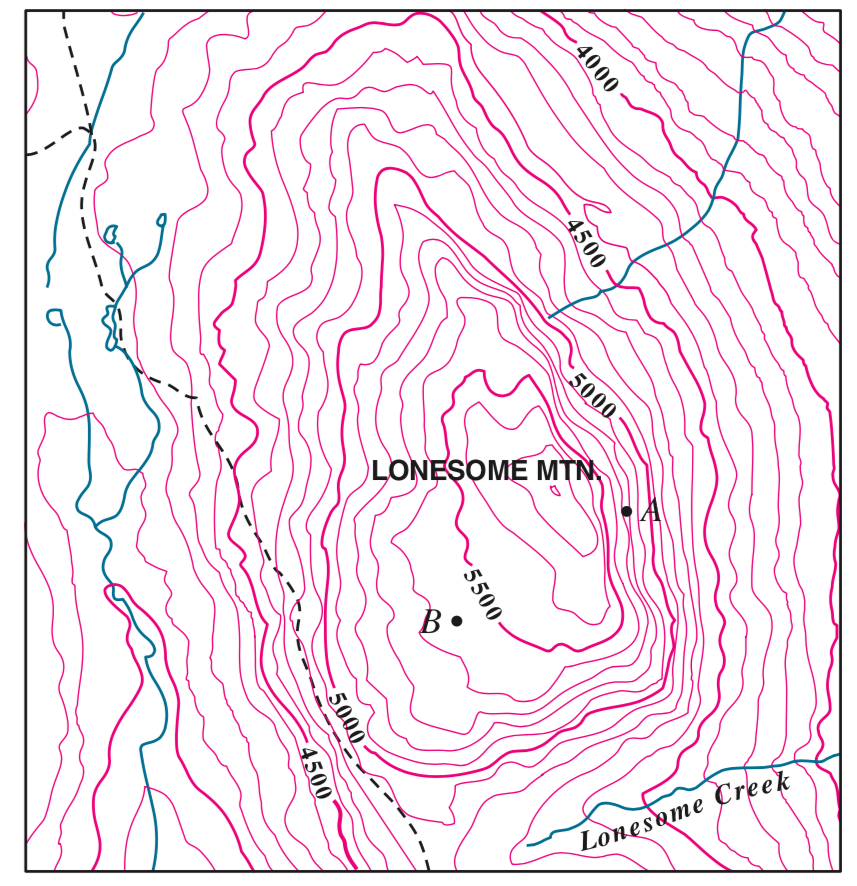
\includegraphics[scale=.2]{lonesome}
   \\
   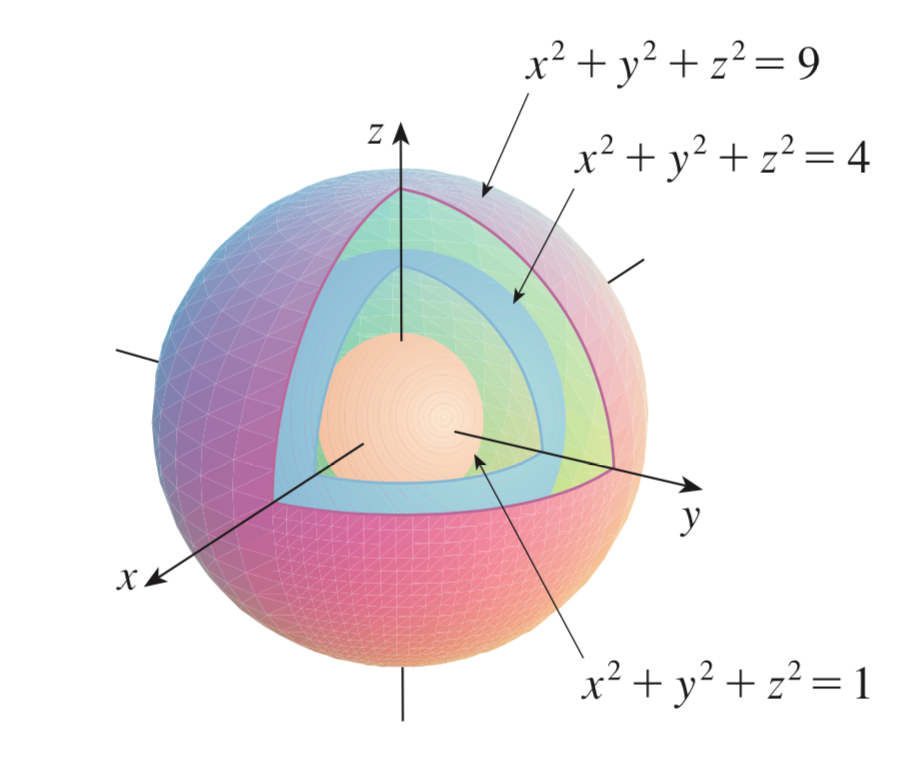
\includegraphics[scale=.2]{level}
   \\
   f(x,y,z) = x^2 + y^2 + z^2
\end{gather*}

\begin{gather*}
   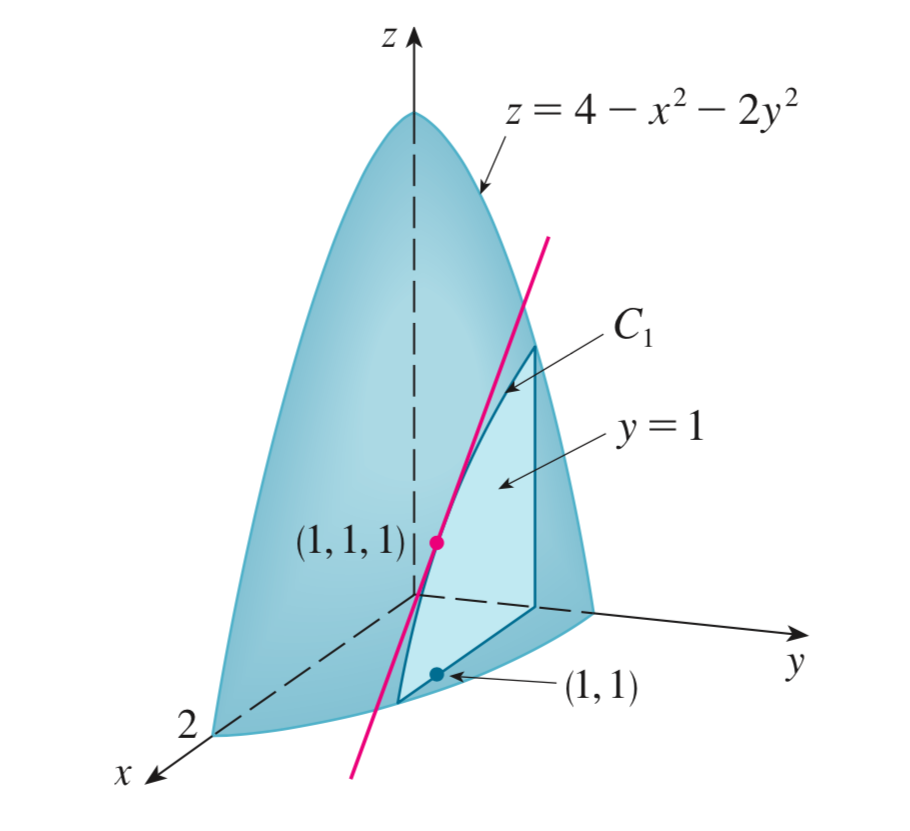
\includegraphics[scale=.2]{partial}
   \\
   \text{The tangent line on $C$ is $\frac{\partial{F}}{\partial{x}}$}
\end{gather*}

\begin{gather*}
   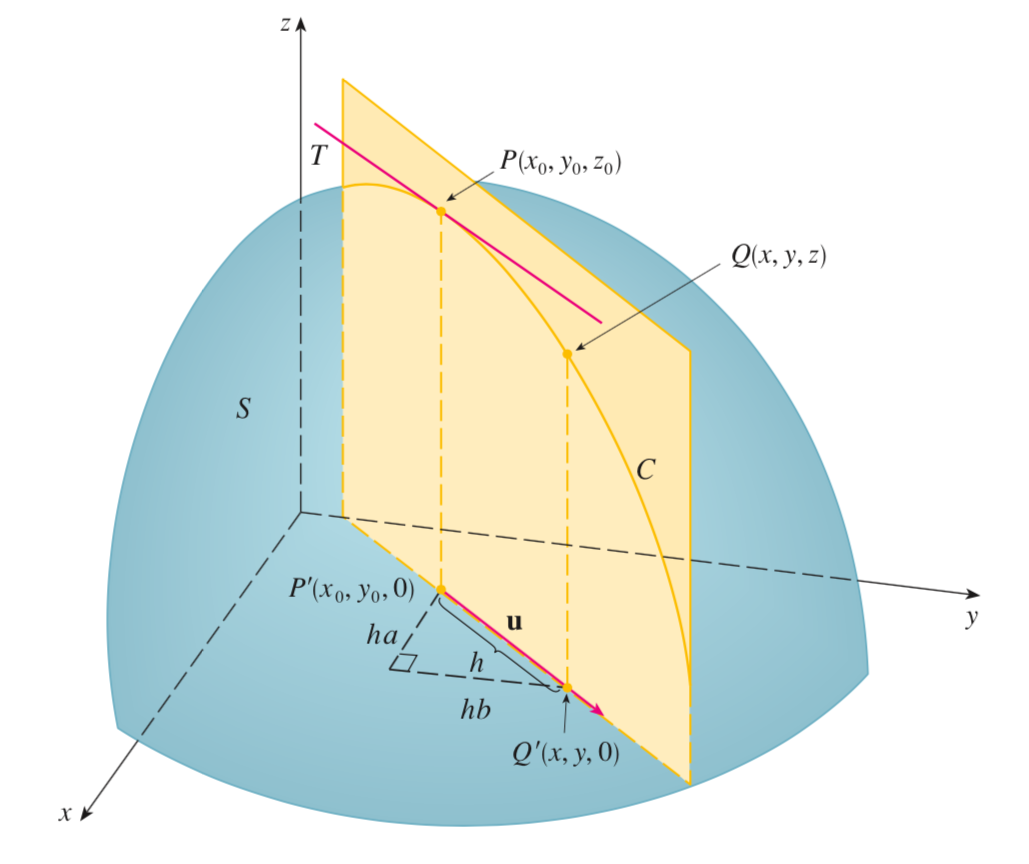
\includegraphics[scale=.2]{directional}
   \\
   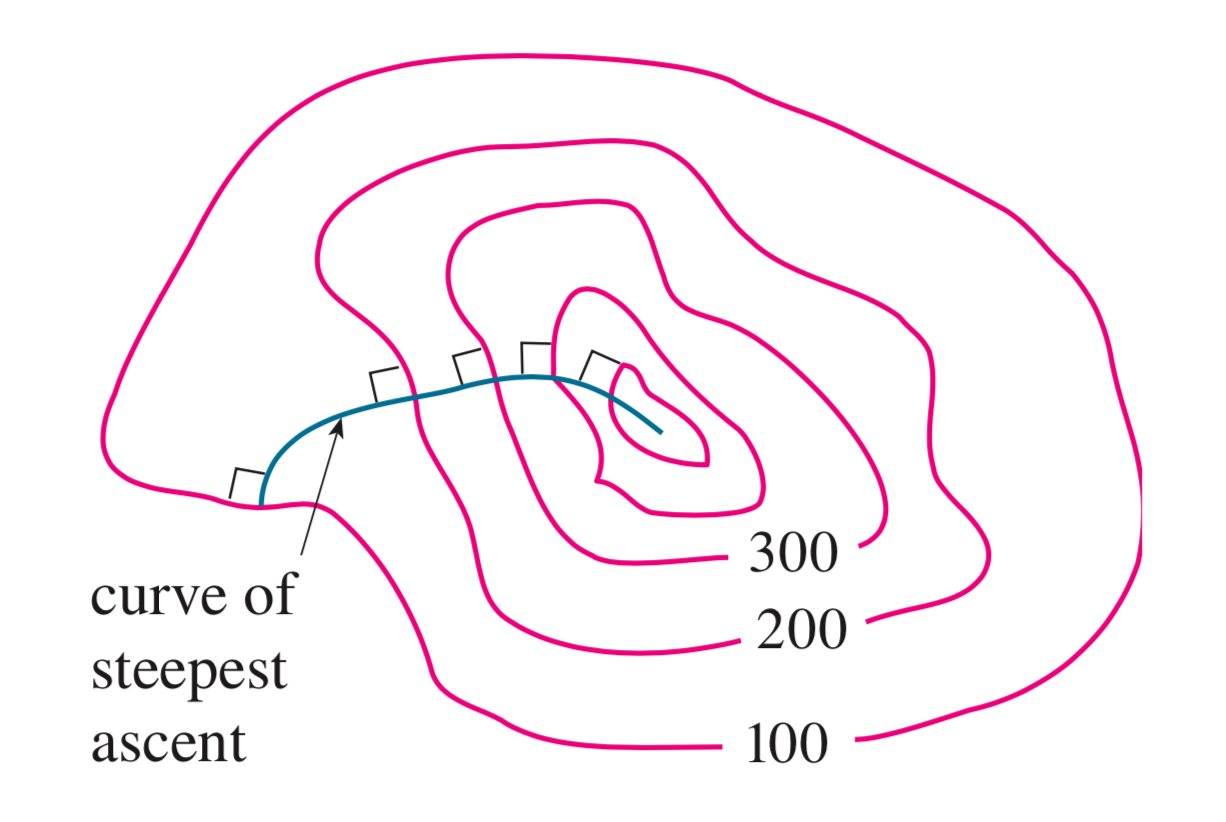
\includegraphics[scale=.2]{steep}
   \\
   \text{The direction of the gradient vector, $\nabla f(x,y,z)$, is the direction of steepest ascent because}
   \\
   \text{$D_u$ is maximized with $\nabla f\cdot\vec{u}$ when $u$ is in the direction of $\nabla f$}
\end{gather*} 

\begin{gather*}
   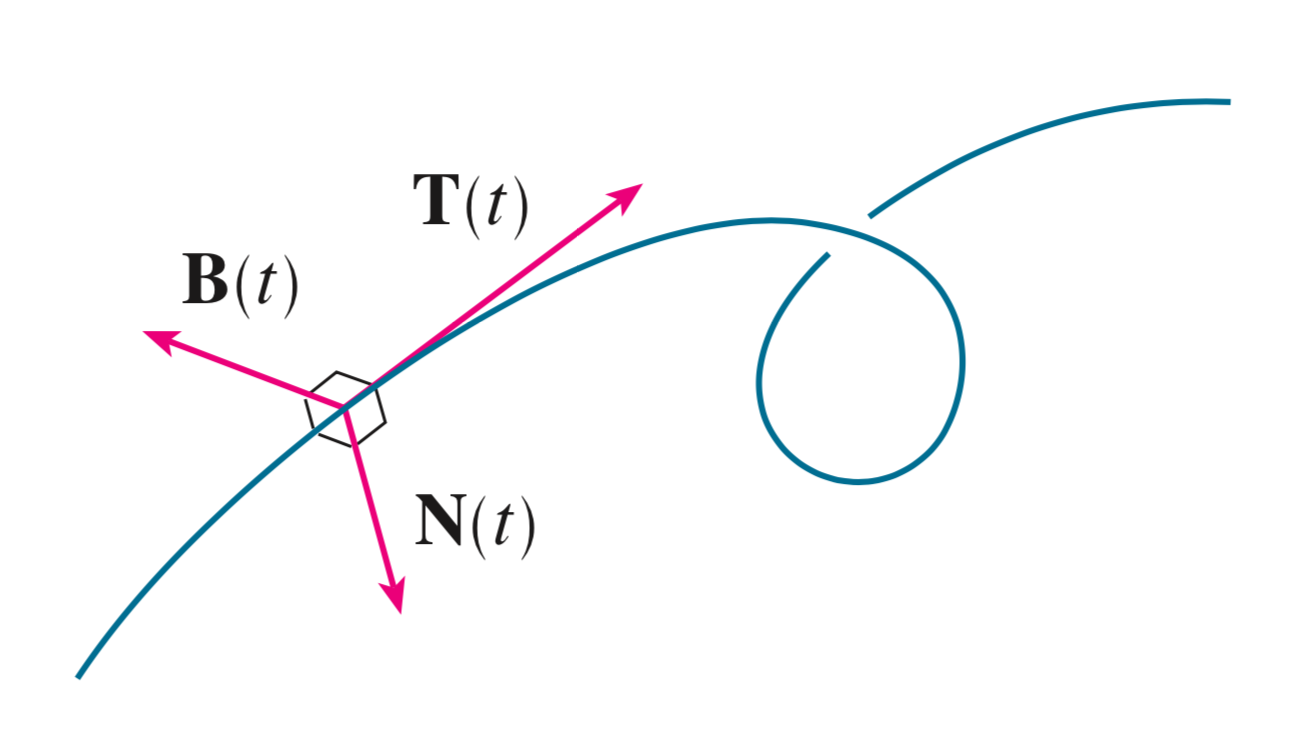
\includegraphics[scale=.13]{TNB}
   \\
   \vec{T(t)} = \frac{\vec{r'(t)}}{|\vec{r'(t)}|} 
   \\
   \vec{N(t)} = \frac{\vec{T'(t)}}{|\vec{T'(t)}|}
   \\
   \vec{B(t)} = \vec{T(t)}\times\vec{N(t)}
   \\
   \kappa = \frac{|d\vec{T}|}{|ds|}
\end{gather*}

\begin{gather*}
    \text{Tangent Plane to a Level Surface}
    \\
    \nabla f(x_0,y_0,z_0)\cdot<x-x_0,y-y_0,z-z_0>=0
    \\
    \text{Tangent Line to a Level Curve}
    \\
    \nabla f(x_0,y_0)\cdot<x-x_0,y-y_0>=0
\end{gather*}
\begin{gather*}
 	   \text{Tangent Plane to a Level Surface}
	    \\
 	   \nabla f(x_0,y_0,z_0)\cdot<x-x_0,y-y_0,z-z_0>=0
 	   \\
 	   \text{Tangent Line to a Level Curve}
	    \\
	    \nabla f(x_0,y_0)\cdot<x-x_0,y-y_0>=0
\end{gather*}
\begin{gather*}
    \text{Curvature Proof}
\end{gather*}
\begin{alignat}{2}
\setcounter{equation}{0}
    T=\frac{r'}{|r'|}                           &\quad &\text{Definition}
    \\
    |r'|=\frac{ds}{dt}                          &\quad &s(t)=\int_a^t|r'(u)|du\text{, First Theorem of Calculus}
    \\
    r'=|r'|T                                    &\quad &\text{1, Algebra}
    \\
    |r'|T=\frac{ds}{dt}T=r'                     &\quad &\text{2, 3, Algebra}
    \\
    r''=\frac{d^2s}{dt^2}T+\frac{ds}{dt}T'      &\quad &\text{4, Product rule}
    \\
    T\times T=0                                 &\quad &\text{Property of cross product}
    \\
    r'\times r''=(\frac{ds}{dt})^2(T\times T')  &\quad &\text{4, 5, 6, } c\Vec{a}\times c\Vec{b}=c^2(\Vec{a}\times \Vec{b})
    \\
    |r'\times r''|=(\frac{ds}{dt})^2|T||T'|sin(\frac{\pi}{2})=(\frac{ds}{dt})^2|T'| &\quad &\text{7, definition of cross, } |T|=1\text{ so, } T\text{ is orthogonal to }T'
    \\
    |T'|=\frac{|r'\times r''|}{(\frac{ds}{dt})^2} &\quad &\text{8, Algebra}
    \\
    |T'|=\frac{|r'\times r''|}{|r'|^2}         &\quad &\text{2, 9, Algebra}
    \\
    \kappa=\frac{|T'|}{|r'|}                    &\quad &\kappa=|\frac{dT}{ds}|\text{ chain rule to }|\frac{\frac{dT}{dt}}{\frac{ds}{dt}}=\frac{|T'|}{|r'|}
    \\
    \kappa=\frac{|r'\times r''|}{|r'|^3}        &\quad &\text{10, 11, Algebra}
\end{alignat}

\begin{gather*}
    \text{Tangential and Normal Components of Acceleration}
\end{gather*}
\begin{alignat}{2}
\setcounter{equation}{0}
    v=|\Vec{\text{v}}(t)|                           &\quad &\text{Definition}
    \\
    \Vec{T}(t)=\frac{\Vec{r'}(t)}{|\Vec{r'}(t)|}=\frac{\Vec{\text{v}}(t)}{|\Vec{\text{v}}(t)}=\frac{\Vec{\text{v}}}{v}                &\quad &\text{Definition, }r'(t)=v(t)
    \\
    \Vec{\text{v}}=v\Vec{T}                         &\quad &\text{2, Algebra}
    \\
    \Vec{\text{v'}}=\Vec{a}=v'\Vec{T}+v\Vec{T'}     &\quad &\text{3, Product rule}
    \\
    \kappa=\frac{|\Vec{T'}|}{|\Vec{r'}|}=\frac{|\Vec{T'}|}{v}    &\quad &\text{Definition, chain rule }\kappa=|\frac{dT}{ds}|=\frac{|\frac{dT}{dt}|}{|\frac{ds}{dt}|}=\frac{|T'|}{|r'|}
    \\
    |\Vec{T'}|=\kappa v                             &\quad &\text{5, Algebra}
    \\
    \Vec{N}=\frac{\Vec{T'}}{|\vec{T'}|}                   &\quad &\text{Definition}
    \\
    \vec{T'}=|\vec{T'}|\vec{N}=\kappa v\vec{N}      &\quad &\text{6, 7, Algebra}
    \\
    \vec{a}=v'\vec{T}+\kappa v^2\vec{N}             &\quad &\text{4, 8, Algebra}
    \\
    \vec{a}=a_T\vec{T}+a_N\vec{N}                   &\quad &\text{Where }a_T=v'\text{ and }a_N=\kappa v^2
\end{alignat}

\begin{gather*}
    \text{Normal Component of Acceleration}
\end{gather*}
\begin{alignat}{2}
\setcounter{equation}{0}
    \Vec{a}=v'\Vec{T}+\kappa v^2\Vec{N}              &\quad &\text{Definition}
    \\
    \Vec{\text{v}}=v\Vec{T}                         &\quad &\text{Definition}
    \\
    \Vec{\text{v}}\cdot\Vec{a}=v\Vec{T}\cdot(v'\Vec{T}+\kappa v^2\Vec{N})   &\quad &\text{1, 2, Substitution}
    \\
    \Vec{\text{v}}\cdot \Vec{a}=vv'\Vec{T}\cdot\Vec{T}+\kappa v^2\Vec{T}\cdot\Vec{N}
    \\
    \Vec{\text{v}}\cdot\Vec{a}=vv'                  &\quad &\text{4, }\Vec{T}\cdot\Vec{T}=1\text{ and }\Vec{N}\cdot\Vec{T}=0
    \\
    a_T=v'=\frac{\Vec{\text{V}}\cdot\Vec{a}}{v}=\frac{r'(t)\cdot r''(t)}{|r'(t)|}   &\quad &\text{5, Definition, Algebra}
    \\
    a_n=\kappa v^2=\frac{|r'(t)\times r''(t)|}{|r'(t)|^3}|r'(t)|^2  &\quad &\text{Previously proved theorem, definitions}
    \\
    a_n=\frac{|r'(t)\times r''(t)|}{|r'(t)|}        &\quad &\text{7, Algebra}
\end{alignat}
\end{document}
